\chapter{User Manual}\label{ch:userManual}
\lstset{basicstyle=\ttfamily}

\section{Installation Requirements}
In this documentation, we make the assumption that you have already installed at least Spark version 1.5.0 and have it configured properly. If you have not performed this step, you can find installation and setup instructions at \url{http://spark.apache.org/downloads.html}.

The next step will be to clone the Git repository of our team. This can be found hosted on Github at: \url{https://github.com/hosamshahin/Spring2016_IR_Project.git}

Finally, you will need to extract the \texttt{small\_data.zip} file that can be found in the\\ \texttt{Spring2016\_IR\_Project/data} directory

\section{Preparing the Server}
In order for some of the Machine Learning libraries in Spark to work, you need to ensure that you have \texttt{libgfortran3} installed.

On a Debian based system, you can run the following command:
\begin{lstlisting}[language=bash]
  $ sudo apt-get install libgfortran3
\end{lstlisting}

Next install Anaconda which is a completely free Python distribution. It includes more than 400 of the most popular Python packages for science, math, engineering, and data analysis. For complete instructions on how to download and install Anaconda go to:

\url{https://www.continuum.io/downloads}

Anaconda is shipped with IPython notebook, a powerful interactive shell for Python.

To set up Spark and IPython to run together and provide a nice web interface, there are a number of things that need to be done.

Begin by creating an IPython profile for PySpark. This can be done using the command:
\begin{lstlisting}[language=bash]
  $ ipython profile create pyspark
\end{lstlisting}

If you are running other IPython profiles, you may want to change the default port. This can be done by modifying \texttt{\texttildelow/.ipython/profile\_pyspark/ipython\_notebook\_config.py}.

You can then change the default port within that file.
\begin{lstlisting}[language=python]
  c = get_config()
  # Simply find this line and change the port value
  c.NotebookApp.port = <your port number>
\end{lstlisting}

Next the following lines need to be placed in \texttt{.bashrc}.
\begin{lstlisting}[language=bash]
  export PYTHONPATH=$SPARK_HOME/python:$PYTHONPATH
  export PYTHONPATH=$SPARK_HOME/python/lib/py4j-0.8.2.1-src.zip:$PYTHONPATH
\end{lstlisting}

After this the \texttt{.bashrc} file should be reloaded by relogging in, or sourcing the \texttt{.bashrc} file.

To run the IPython server you should run the following command from within the cloned git repository, replacing <IP> with the IP address of your server.
\begin{lstlisting}[language=bash]
  ipython notebook --profile=pyspark --no-browser --ip <IP>
\end{lstlisting}

You can then navigate to <IP>:<PORT> in your browser to get access to the IPython notebook. By default the port will be 8888.

\section{Using the IPython Notebook}

Once the IPython notebook has been opened in the browser, open the \texttt{Tweets\_Classification-V2.ipynb} IPython notebook. You should see something similar to Figure \ref{fig:ipy_notebook}.

\begin{figure}[th!]
	\centering
	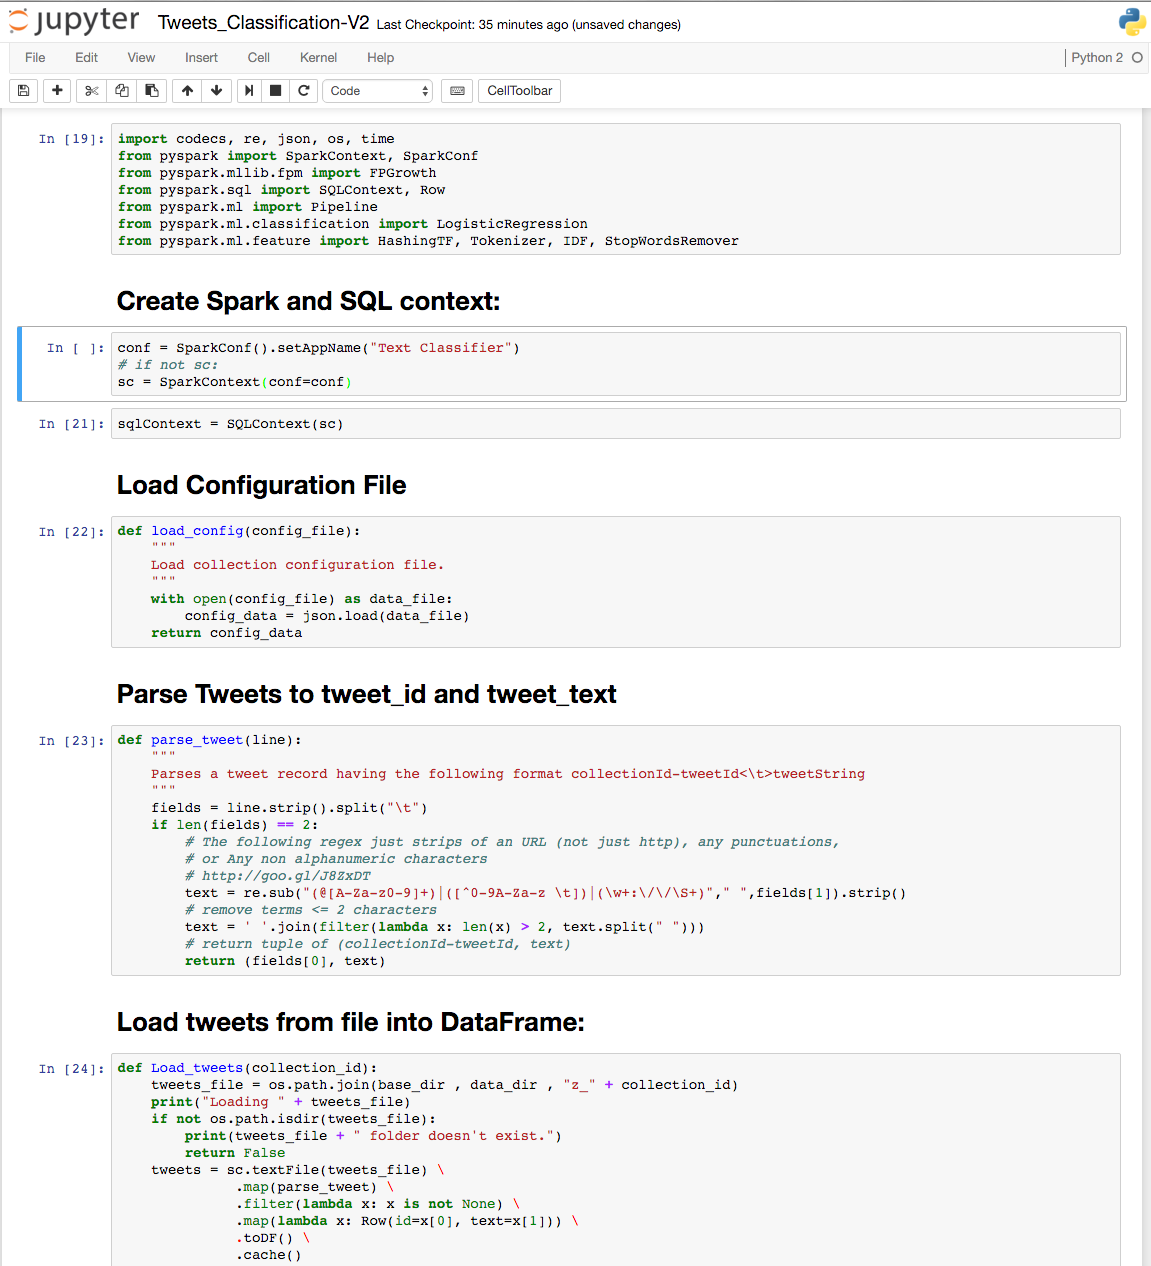
\includegraphics[width=\textwidth]{figures/IPython_Tweet_Classification}
    \caption{IPython notebook}\label{fig:ipy_notebook}
\end{figure}

In order to use the script, you will need to modify the \texttt{base\_dir} variable in cell 10. Set this to point at the \texttt{data} directory.

\subsection{Using the Configuration File}

To go further in using the script, you may need to make modifications to the \texttt{collections\_config.json} file under \texttt{data}; see Figure \ref{fig:collection_config}. The provided configuration file is already configured to work with the six small datasets that were assigned to the groups at the start of the semester. However, the frequent patterns (FP) field has not been properly configured. This will need to be done for each collection as you work through the tutorial.

\begin{figure}[th!]
	\centering
	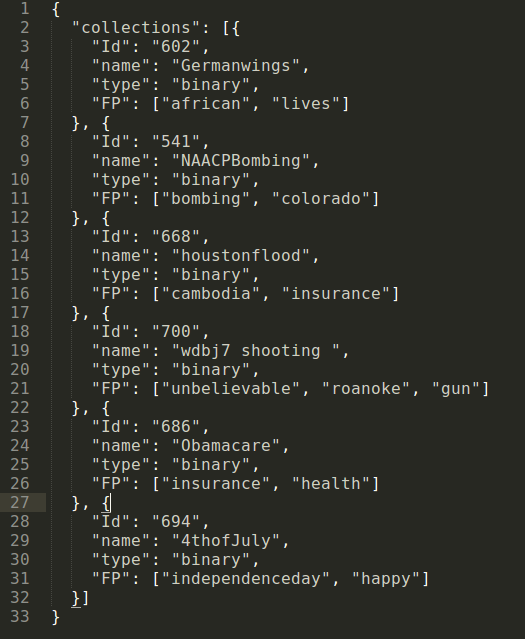
\includegraphics[width=0.5\textwidth]{figures/collection_config}
    \caption{Collections configuration file}\label{fig:collection_config}
    \foxComment{The FP entries seem odd. (HS: I've changed the configuration file image with a new one that has more meaningful terms)

Was there overfitting to an odd positive set?}
\end{figure}

%At this point the only section of the file that needs to be worried about is the first collection object. That is being used for the binary classifications we are currently using. The second object will be used for multiclass classification in the future.

To classify your data, you need to specify the table ID of your collection in the \texttt{collections\_config.json} configuration file. You should model your entry off of one of the sample entries in the file, or modify a sample directly. It is also suggested that you update the name field to the name of your collection. At the moment, don't worry about the FP values.

\subsection{Selecting a Frequent Pattern}

After setting the configuration file, begin at the first cell and press Shift + Enter to execute each cell in order. Continue this until you reach ``Manually choose frequent patterns and write them in the configuration file.''

You will now need to open each of the frequent pattern output files located at:\\
\texttt{data/FPGrowth/<<timestamp>>\_<<collectionId>>\_<<collection\_name>>.txt}

You should now inspect the file for the tokens frequently found together. Look for high frequency patterns. Choose a pattern that seems highly relevant to your collection. We suggest a pattern of two to four words to strike a balance between over and under specification.

Take the pattern and copy it as the value of ``FP'' in the configuration file.

\begin{figure}[th!]
  \centering
  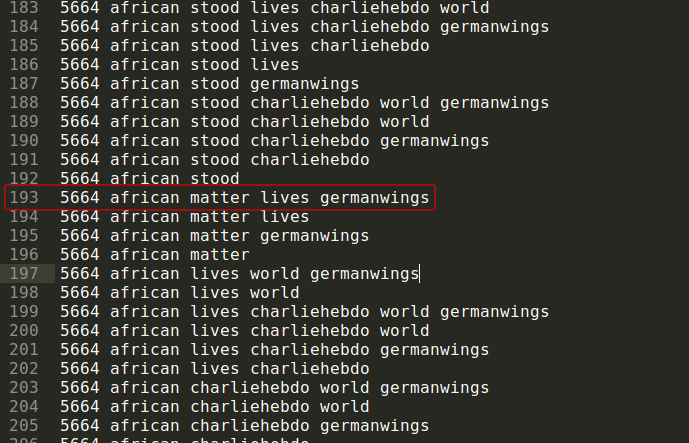
\includegraphics[width=0.5\textwidth]{figures/Germanwings_FP.png}
    \caption{Frequent Patterns Mining algorithm output file for Germanwings collection}\label{fig:collection_config}
\end{figure}

\foxComment{Can you give examples? (HS: this is an example of FPM output of Germainwings tweets collection)}

\subsection{Building a Training Set}

After the frequent pattern has been selected and input into the configuration file, continue to step through the script using Shift + Enter  in each cell.

This will take you through the process of building a training set by identifying a positive sample set and a negative sample set and placing those into a DataFrame.

\subsection{Training a Classifier}

Further progression through the script will actually use the training data constructed in the last step to train a logistic regression classifier.

\subsection{Running the Classifier}

Finally, apply the classification model to our test data and provide a prediction of relevance (1.0) or non-relevance (0.0) for each tweet in the test data. This data can be found in the \texttt{predictions} directory and has the same name formatting as the frequent pattern output files.

\foxComment{HS: Figure~\ref{fig:histograms} shows the different histograms for the small data sets where higher probability means more likly a tweet to be relavant to the collection}

\begin{figure}[t!] % "[t!]" placement specifier just for this example
	\begin{subfigure}{0.50\textwidth}
		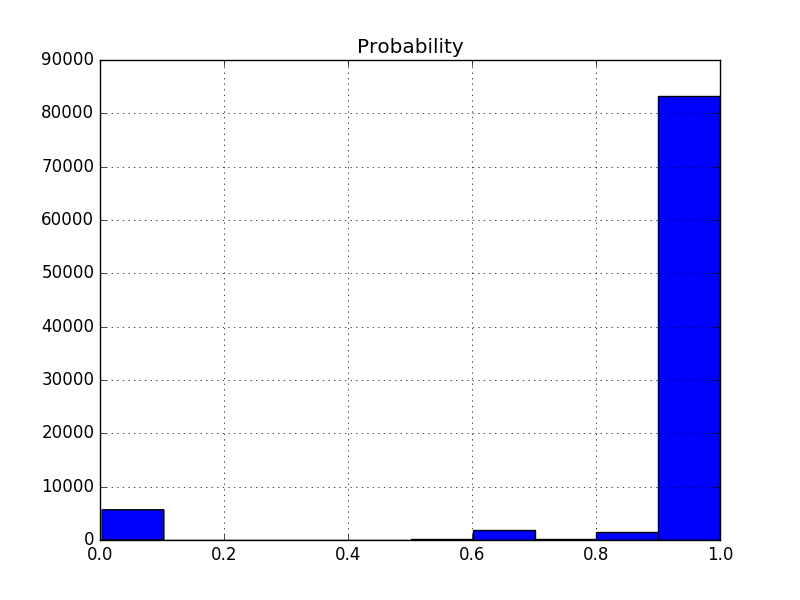
\includegraphics[width=\linewidth]{figures/Germanwings.png}
		\caption{Germanwings} \label{fig:a}
	\end{subfigure}\hspace*{\fill}
	\begin{subfigure}{0.50\textwidth}
		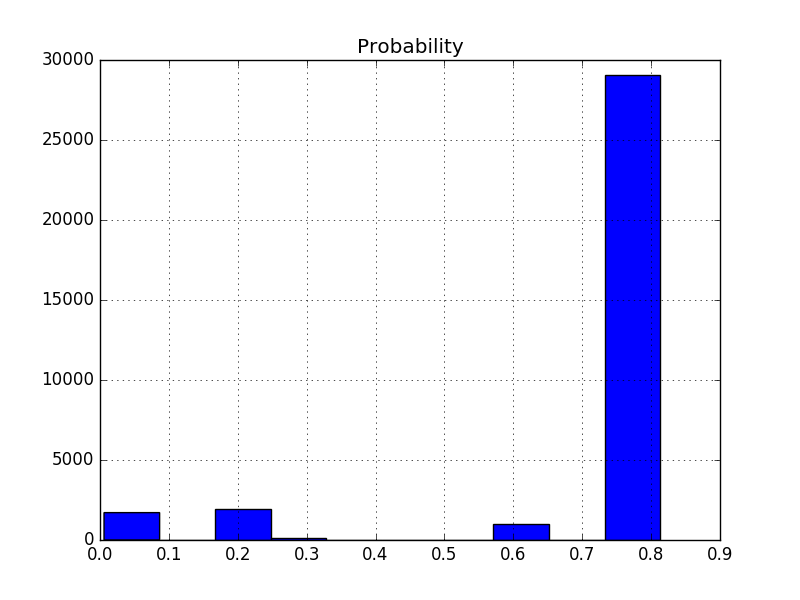
\includegraphics[width=\linewidth]{figures/NAACPBombing.png}
		\caption{NAACPBombing} \label{fig:b}
	\end{subfigure}

	\medskip
	\begin{subfigure}{0.50\textwidth}
		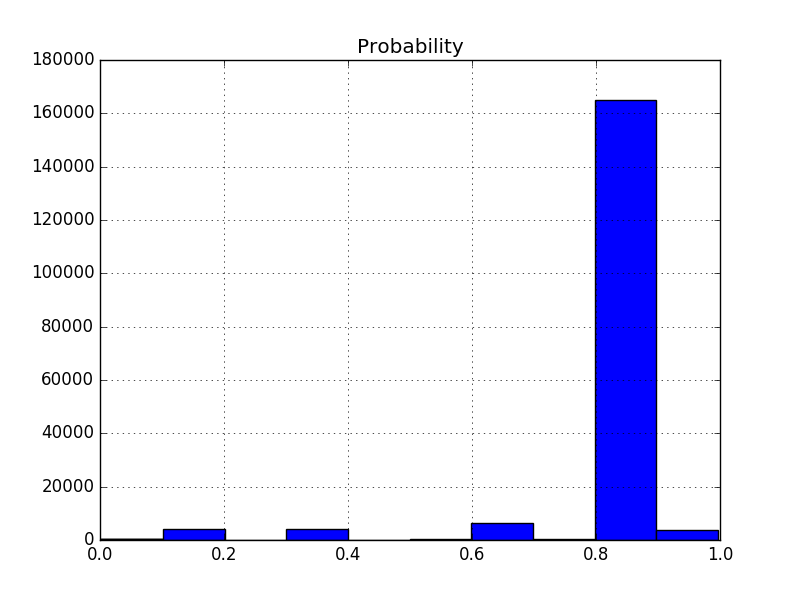
\includegraphics[width=\linewidth]{figures/Obamacare.png}
		\caption{Obamacare} \label{fig:c}
	\end{subfigure}\hspace*{\fill}
	\begin{subfigure}{0.50\textwidth}
		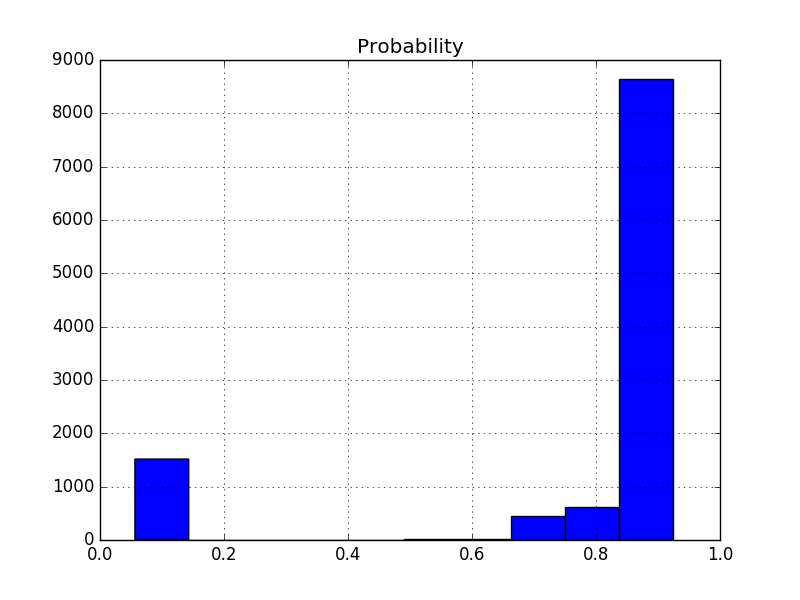
\includegraphics[width=\linewidth]{figures/wdbj7shooting.png}
		\caption{wdbj7shooting} \label{fig:d}
	\end{subfigure}

	\medskip
	\begin{subfigure}{0.50\textwidth}
		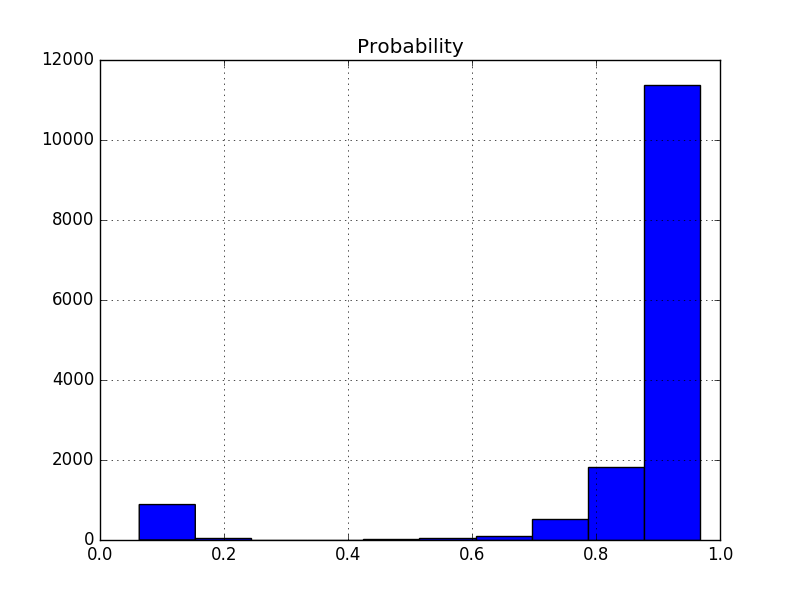
\includegraphics[width=\linewidth]{figures/houstonflood.png}
		\caption{houstonflood} \label{fig:e}
	\end{subfigure}\hspace*{\fill}
	\begin{subfigure}{0.50\textwidth}
		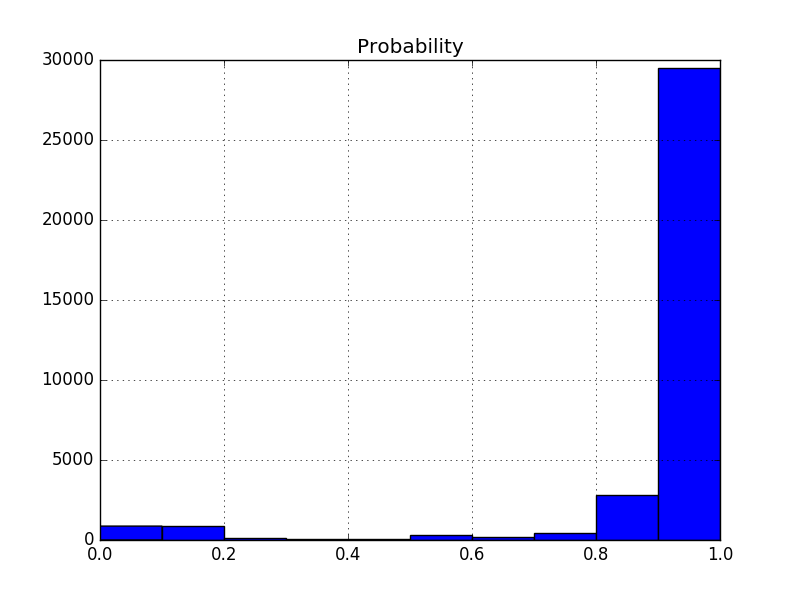
\includegraphics[width=\linewidth]{figures/fourthofJuly.png}
		\caption{4thofJuly} \label{fig:f}
	\end{subfigure}

	\caption{Histograms for the small collections of tweets } \label{fig:histograms}
\end{figure}

A cross-reference to Figure~\ref{fig:histograms}, and a cross-reference to Subfigure~\ref{fig:e}.

% Here is the introduction. The next chapter is chapter~\ref{ch:ch2label}.


% a new paragraph


% \section{Examples}
% You can also have examples in your document such as in example~\ref{ex:simple_example}.
% \begin{example}{An Example of an Example}
%   \label{ex:simple_example}
%   Here is an example with some math
%   \begin{equation}
%     0 = \exp(i\pi)+1\ .
%   \end{equation}
%   You can adjust the colour and the line width in the {\tt macros.tex} file.
% \end{example}

% \section{How Does Sections, Subsections, and Subsections Look?}
% Well, like this
% \subsection{This is a Subsection}
% and this
% \subsubsection{This is a Subsubsection}
% and this.

% \paragraph{A Paragraph}
% You can also use paragraph titles which look like this.

% \subparagraph{A Subparagraph} Moreover, you can also use subparagraph titles which look like this\todo{Is it possible to add a subsubparagraph?}. They have a small indentation as opposed to the paragraph titles.

% \todo[inline,color=green]{I think that a summary of this exciting chapter should be added.}